% Section 5: Numerical Studies
\begin{block}{\fontsize{46}{54}\selectfont 5. Numerical Studies}

{\fontsize{40}{48}\selectfont \textbf{A) Solver Comparison (HGS vs Gurobi)}}

\vspace{0.3cm}
\noindent
\begin{minipage}[t]{0.26\linewidth}
    \vspace{0pt}
    {\fontsize{34}{42}\selectfont \textbf{Small Instances}}\\[0.15cm]
    {\fontsize{28}{34}\selectfont $|S|\le 15$, $|K|{=}|R|{=}1$}\\[0.1cm]
    {\fontsize{28}{34}\selectfont All solved to \textbf{optimality}.}
    
    \vspace{0.3cm}
    {\fontsize{28}{34}\selectfont CPU times (s): Gurobi vs HGS}
    
    \vspace{0.25cm}
    \renewcommand{\arraystretch}{1.25}
    {\fontsize{26}{32}\selectfont
    \begin{tabular*}{\linewidth}{@{\extracolsep{\fill}}c r r@{}}
        \toprule
        \multicolumn{3}{c}{\textbf{$|S|=6$}} \\
        \midrule
        inst. & Gurobi & HGS \\
        \midrule
        1 & 13.41 & 6.29 \\
        2 & 13.85 & 5.75 \\
        3 & 66.97 & 6.22 \\
        4 & 2.29  & 3.63 \\
        5 & 22.29 & 4.84 \\
        \bottomrule
    \end{tabular*}}
    
    \vspace{0.2cm}
    {\fontsize{26}{32}\selectfont
    \begin{tabular*}{\linewidth}{@{\extracolsep{\fill}}c r r@{}}
        \toprule
        \multicolumn{3}{c}{\textbf{$|S|=10$}} \\
        \midrule
        inst. & Gurobi & HGS \\
        \midrule
        1 & 928.50   & 3.87 \\
        2 & 1409.89  & 5.27 \\
        3 & 13768.72 & 3.02 \\
        4 & 2404.03  & 5.16 \\
        5 & 4172.75  & 4.17 \\
        \bottomrule
    \end{tabular*}}
    
    \vspace{0.2cm}
    {\fontsize{26}{32}\selectfont
    \begin{tabular*}{\linewidth}{@{\extracolsep{\fill}}c r r@{}}
        \toprule
        \multicolumn{3}{c}{\textbf{$|S|=15$}} \\
        \midrule
        inst. & Gurobi & HGS \\
        \midrule
        1 & 2602.24 & 7.80 \\
        2 & 4209.67 & 4.89 \\
        3 & 6283.58 & 4.72 \\
        4 & 3374.38 & 5.32 \\
        5 & 2371.40 & 5.08 \\
        \bottomrule
    \end{tabular*}}
\end{minipage}%
\hspace{0.01\linewidth}%
\vrule width 1.5pt%
\hspace{0.01\linewidth}%
\begin{minipage}[t]{0.70\linewidth}
    \vspace{0pt}
    {\fontsize{34}{42}\selectfont \textbf{Large Instances (Scalability):} $|S|=60$--500, $K\in\{1,2\}$, $R\in\{1,2\}$.}
    
    \vspace{0.25cm}
    \renewcommand{\arraystretch}{1.25}
    \setlength{\tabcolsep}{10pt}
    {\fontsize{26}{32}\selectfont
    \begin{tabular*}{\linewidth}{@{\extracolsep{\fill}}c rrr rrr rrr rrr rr@{}}
        \toprule
        & \multicolumn{3}{c}{\boldmath$K{=}1, R{=}1$} & \multicolumn{3}{c}{\boldmath$K{=}1, R{=}2$} & \multicolumn{3}{c}{\boldmath$K{=}2, R{=}1$} & \multicolumn{3}{c}{\boldmath$K{=}2, R{=}2$} & \multicolumn{2}{c}{\textbf{CPU (s)}} \\
        \cmidrule(lr){2-4} \cmidrule(lr){5-7} \cmidrule(lr){8-10} \cmidrule(lr){11-13} \cmidrule(lr){14-15}
        $|S|$ & $O_{\text{H}}$ & $O_{\text{G}}$ & Gap & $O_{\text{H}}$ & $O_{\text{G}}$ & Gap & $O_{\text{H}}$ & $O_{\text{G}}$ & Gap & $O_{\text{H}}$ & $O_{\text{G}}$ & Gap & Grb & HGS \\
        \midrule
        \multicolumn{15}{c}{\textbf{$T=2$ h}} \\
        \midrule
        60  & 2581 & 2605 & 0.9 & 2494 & 2533 & 1.6 & 2401 & 3582 & 33.0 & 2325 & 3518 & 33.9 & 7200 & 6--11 \\
        90  & 4038 & 4511 & 10.5 & 3942 & 4159 & 5.2 & 3862 & 4511 & 14.4 & 3769 & 4489 & 16.0 & 7200 & 9--13 \\
        120 & 4303 & 5114 & 15.9 & 4238 & 5104 & 17.0 & 4168 & 5114 & 18.5 & 4097 & 5104 & 19.7 & 7200 & 9--16 \\
        200 & 7821 & 8657 & 9.7 & 7720 & 8657 & 10.8 & 7642 & 8657 & 11.7 & 7561 & 8657 & 12.7 & 7200 & 12--24 \\
        300 & 11169 & 11717 & 4.7 & 11058 & 11717 & 5.6 & 10989 & 11717 & 6.2 & 10888 & 11717 & 7.1 & 7200 & 17--34 \\
        400 & 14281 & 15069 & 5.2 & 14179 & 15061 & 5.9 & 14169 & 15069 & 6.0 & 14059 & 15061 & 6.7 & 7200 & 25--44 \\
        500 & 18962 & 19794 & 4.2 & 18793 & 19785 & 5.0 & 18752 & 19794$^\dagger$ & 5.3 & 18613 & 19785$^\dagger$ & 5.9 & 7200 & 27--51 \\
        \midrule
        \multicolumn{15}{c}{\textbf{$T=3$ h}} \\
        \midrule
        60  & 2433 & 3554 & 31.5 & 2365 & 3507 & 32.6 & 2265 & 3582 & 36.8 & 2214 & 3507 & 36.9 & 7200 & 10--14 \\
        90  & 3903 & 4504 & 13.3 & 3779 & 4481 & 15.7 & 3705 & 4504 & 17.7 & 3607 & 4481 & 19.5 & 7200 & 10--20 \\
        120 & 4203 & 5114 & 17.8 & 4107 & 5104 & 19.5 & 4024 & 5114 & 21.3 & 3952 & 5104 & 22.6 & 7200 & 9--18 \\
        200 & 7695 & 8657 & 11.1 & 7575 & 8657 & 12.5 & 7471 & 8657 & 13.7 & 7394 & 8657 & 14.6 & 7200 & 14--28 \\
        300 & 11024 & 11716 & 5.9 & 10901 & 11716 & 7.0 & 10830 & 11716 & 7.6 & 10693 & 11716 & 8.7 & 7200 & 18--44 \\
        400 & 14138 & 15069 & 6.2 & 14010 & 15061 & 7.0 & 13969 & 15069$^\dagger$ & 7.3 & 13852 & 15061$^\dagger$ & 8.0 & 7200 & 22--56 \\
        500 & 18818 & 19794 & 4.9 & 18596 & 19785$^\dagger$ & 6.0 & 18572 & 19794$^\dagger$ & 6.2 & 18407 & 19785$^\dagger$ & 7.0 & 7200 & 22--62 \\
        \bottomrule
    \end{tabular*}}
    
    \vspace{0.3cm}
    % Two-column layout for Setup/Symbols and Summary - equal height boxes
    \noindent
    \begin{minipage}[t]{0.485\linewidth}
        \vspace{0pt}
        \colorbox{DarkSlate!8}{\parbox[t][8.5cm][t]{0.96\linewidth}{
            \vspace{0.2cm}
            {\fontsize{28}{34}\selectfont \textbf{Setup \& Notation}}
            
            \vspace{0.2cm}
            {\fontsize{24}{30}\selectfont
            $\bullet$ $CPU^{\text{max}}=7200$ s time limit, 20 runs per instance\\[0.15cm]
            $\bullet$ Repositioning time budget $T\in\{2,3\}$ hours\\[0.15cm]
            $\bullet$ $O_{\text{H}}$: HGS objective (avg. over 20 runs)\\[0.15cm]
            $\bullet$ $O_{\text{G}}$: Gurobi upper bound\\[0.15cm]
            $\bullet$ Gap $= 100\times(O_{\text{G}}-O_{\text{H}})/O_{\text{G}}$\\
            $\bullet$ \colorbox{red!15}{$^\dagger$ Gurobi ran out of memory (64GB)}
            }
        }}
    \end{minipage}%
    \hspace{0.02\linewidth}%
    \begin{minipage}[t]{0.495\linewidth}
        \vspace{0pt}
        \colorbox{AccentGold!22}{\parbox[t][8.5cm][t]{0.98\linewidth}{
            \vspace{0.2cm}
            {\fontsize{28}{34}\selectfont \textbf{Key Findings}}
            
            \vspace{0.2cm}
            {\fontsize{24}{30}\selectfont
            \textbf{Small instances} ($|S|\le 15$):\\[0.15cm]
            \ding{51} HGS matches \textbf{optimal} solutions in all cases\\[0.15cm]
            \ding{51} HGS: \textbf{3--8 seconds} vs Gurobi: \textbf{minutes--hours}\\[0.3cm]
            \textbf{Large instances} ($|S|=60$--500):\\[0.15cm] 
            \ding{51} HGS improves Gurobi UB by up to \textbf{33.9\%} within \textbf{6--62 seconds}\\[0.15cm]
            \ding{51} Gurobi hits 2h time limit to find a worse solution or crashes (64GB)
            }
        }}
    \end{minipage}
\end{minipage}

\vspace{0.4cm}
\hrule
\vspace{0.4cm}

{\fontsize{40}{48}\selectfont \textbf{B) When Are On-Site Repairers Cost-Effective?}}

\vspace{0.3cm}
\noindent
\begin{minipage}[t][22cm][t]{0.52\linewidth}
    \vspace{0pt}
    {\fontsize{34}{42}\selectfont Cost-effectiveness $\nu$ vs repair time (selected $\ell$ values):}
    
    \vspace{0.3cm}
    \centering
    \begin{tabular}{@{}cc@{}}
        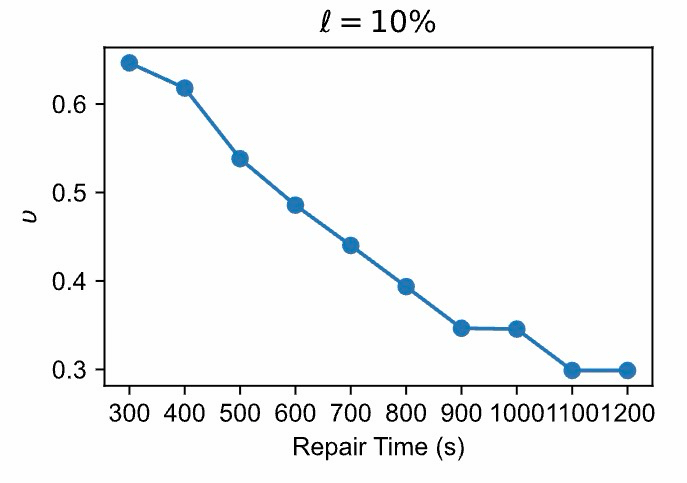
\includegraphics[width=0.48\linewidth]{figures/cost_effectiveness_l10.png} &
        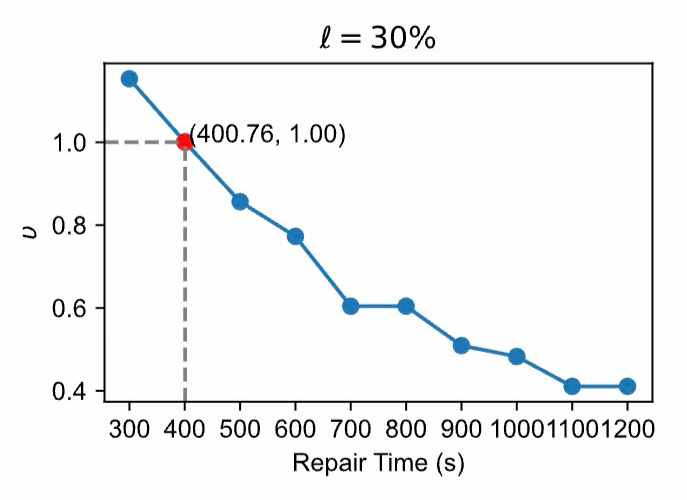
\includegraphics[width=0.48\linewidth]{figures/cost_effectiveness_l30.png} \\[0.3cm]
        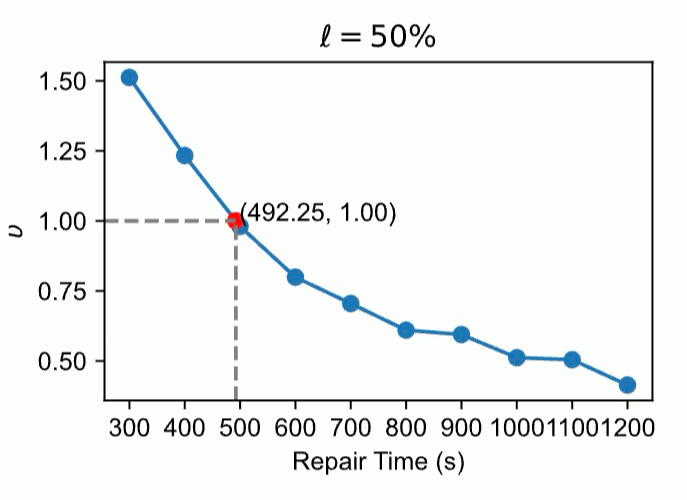
\includegraphics[width=0.48\linewidth]{figures/cost_effectiveness_l50.png} &
        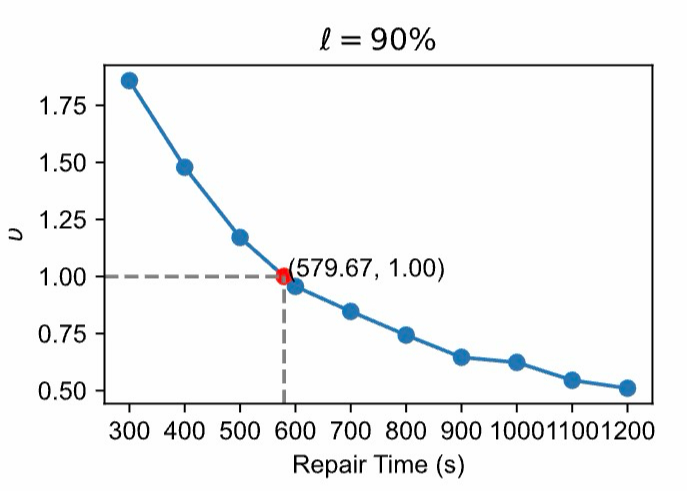
\includegraphics[width=0.48\linewidth]{figures/cost_effectiveness_l90.png} \\
    \end{tabular}
\end{minipage}%
\hspace{0.02\linewidth}%
\begin{minipage}[t][22cm][s]{0.44\linewidth}
    % Match the title line height from left column
    \vspace{1.8cm}
    
    \colorbox{HKUGreen!10}{\parbox{0.96\linewidth}{
        \vspace{0.3cm}
        {\fontsize{40}{48}\selectfont \textbf{Cost-Effectiveness Indicator}}
        
        \vspace{0.55cm}
        \begin{center}
        {\fontsize{48}{58}\selectfont $\displaystyle \nu = \frac{c^p \cdot \Delta F}{\varpi \cdot T/3600}$}
        \end{center}
        
        \vspace{0.55cm}
        {\fontsize{40}{48}\selectfont
        $\bullet$ $\Delta F$: dissatisfaction reduction\\[0.5cm]
        $\bullet$ $c^p$: penalty cost per unit dissatisfaction\\[0.5cm]
        $\bullet$ $\varpi$: repairer hourly wage\\[0.5cm]
        $\bullet$ $\nu$ measures \textbf{benefit per wage}
        }
        \vspace{0.3cm}
    }}
    
    \vspace{0.8cm}
    
    \colorbox{AccentGold!20}{\parbox{0.96\linewidth}{
        \vspace{0.3cm}
        {\fontsize{40}{48}\selectfont \textbf{Key Findings}}
        
        \vspace{0.35cm}
        {\fontsize{40}{48}\selectfont
        \ding{51} \textbf{Low $\ell$ ($\le 20\%$):} repairers \textbf{never} pay off\\[0.15cm]
        \hspace{0.6cm}{\fontsize{40}{48}\selectfont (curves always below $\nu=1$)}\\[0.65cm]
        \ding{51} \textbf{Higher $\ell$} $\Rightarrow$ larger tolerance for\\[0.15cm]
        \hspace{0.6cm}{\fontsize{40}{48}\selectfont slower repairs (\textbf{401--600 s})}\\[0.65cm]
        \ding{51} \textbf{Practical rule:}\\[0.55cm]
        \hspace{0.6cm}{\fontsize{40}{48}\selectfont Deploy repairers when $\ell \ge 30\%$}\\[0.15cm]
        \hspace{0.6cm}{\fontsize{40}{48}\selectfont and repair time $\lesssim 7$--10 min}
        }
        \vspace{0.3cm}
    }}
    
    \vspace{0pt}
\end{minipage}

\end{block}
